\subsection{Vulnerabilità}

\begin{frame}
    Le vulnerabilità trovate negli anni nel crittosistema sono le seguenti.

    Alcune di queste sono di facile soluzione perchè riguardano il lato hardware del lettore,
    per cui, a fronte di un costo maggiore, è possibile migliorarne le capacità.
\end{frame}

\begin{frame}
    \scriptsize
    \begin{itemize}
        \item <1-> Utilizzo di chiavi a 48 bit: Possibili attacchi BruteForce \cite{courtois2008algebraic}
        \item <2-> RNG del tag non è crittograficamente sicuro. infatti è un LFSR (a 16 bit) con condizione iniziale costante.
        \begin{itemize} \scriptsize
            \item <3-> Consegue che lo stato è prevedibile e dipende dal tempo trascorso dal poweron~\cite{garcia2008dismantling}\cite{courtois2008algebraic}
            \item <4-> Inoltre i numeri casuali sono generati a partire da 16 bit del registro 
            \item <5-> in particolare i numeri sono generati ad ogni ciclo di clock del tag, quindi la precisione del attaccante deve limitarsi a quanti di 10 microsecondi (106kHz) e la sequenza di numeri i ripete ogni 65535 iterazioni (0.6s)
        \end{itemize}
        \item <6-> L'RNG dei lettori viene aggiornato solamente ad ogni nuova autenticazione~\cite{garcia2008dismantling}
        \item <7-> La funzione di filtraggio del LFSR usa 20bit del registro e sono solo bit in posizione dispari
        \item <8-> LFSR State Recovery
        \item <9-> LFSR Rollback
        \item <10-> i bit di parità sono computati sul plaintext e poi inviati non cifrati
        \item <11-> nested authentication attacks
    \end{itemize}
\end{frame}

\begin{frame}
    \frametitle{Bit di parità}
    \label{sec:parity-enc}
    Ulteriore vulnerabilità dell'implementazione sta nel fatto che il livello di trasmissione fisica richiede 
    un invio di un bit di parità ogni 8 bit di dato \pause

    IL BIT DI PARITÀ È QUINDI INVIATO CIFRATO \textbf{CONDIVIDENDO IL BIT DEL KEYSTREAM} MA VIENE \textbf{CALCOLATO SUL PLAINTEXT}\cite{Courtois2009TheDS}\pause

    \begin{figure}
        \centering
        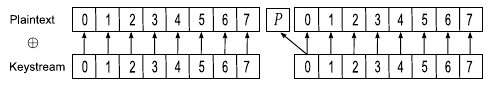
\includegraphics[width=0.8\textwidth]{keystream-parity.png}
        \caption{Assegnazione dei bit di cifratura tra dati e bit di parità}
        \label{fig:keystream-parity}
    \end{figure}
\end{frame}
\note{
    Questo permette di avere informazioni sul keystream (almeno su un bit ogni 8) ed è una proprietà utilizzabile per ridurre lo spazio di ricerca negli attacchi Nested authentication (vedi slide~\ref{sec:nested-auth})
}

\begin{frame}
    \frametitle{Errori di trasmissione}
    \label{sec:parity-bit-vuln}
    Secondo il protocollo ISO14443a ogni 8 bit di dati deve essere inviato un bit di parità.\pause

    Il tag riceve una sequenza di dati con bit di parità invalidi $\implies$ Nessuna risposta da parte del tag\pause

    Il tag riceve una sequenza con bit di parità corretti ma la verifica della risposta alla challenge non ha successo $\implies$ NACK\pause

    {\large IL NACK È CIFRATO MA È UN TESTO CONOSCIUTO}
\end{frame}
\note{
}